\newpage
\chapter{Badania}
%\textbf{Przerzucone z wcześniejszych rozdziałów:}
%\begin{itemize}
%\item W przypadku wszystkich opisanych w tym rozdziale algorytmów za \emph{warunkiem stopu} można rozumieć wykonanie z góry określonej maksymalnej liczby iteracji pętli lub brak poprawy najlepszego rozwiązania w pewnej liczbie ostatnich przebiegów algorytmu. 
%\item Do ustawiana elitismu w genetycznym i memetycznym - Tak również postąpiono w trakcie przeprowadzania badań w ramach tej pracy - wykorzystano domyślny w pakiecie \emph{GA} rozmiar grupy chronionych osobników wynoszący 5\% populacji.
%\end{itemize}


\section{Specyfikacja funkcji testowych}
Znajdowanie coraz lepszych metod rozwiązywania problemów optymalizacyjnych oraz ich testowanie jest zagadnieniem na tyle powszechnym, że powstały w tym celu narzędzia to ułatwiające. Dzięki ujednoliceniu sposobu badań wydajności algorytmów możliwe jest porównywanie ich na płaszczyźnie tych samych problemów. Jednym z pakietów języka \emph{R} powstałym w tym celu jest \emph{globalOptTests} \cite{globalOptTestsPackage}. Stanowi go zbiór kilkunastu funkcji o różnej liczbie parametrów. Każda z nich dodatkowo opisana jest dziedziną wartości poszczególnych argumentów oraz wartością funkcji w ekstremum. Wszystkie problemy zawarte w pakiecie są zadaniami znalezienia \emph{minimum} globalnego.
\par
Na potrzeby przeprowadzenia badań porównawczych różnych algorytmów wybrano z pakiety \emph{globalOptTests} 3 funkcje, które zostaną opisane poniżej. Reprezentują one problemy  optymalizacyjne o różnej wymiarowości. 
\subsection{Funkcja Schaffer1}
\begin{itemize}
\item wzor
\item wykres, bo 2D
\item dziedzina argumentow
\item optimum: 0, w początku układu współrzędnych
\item cechy: wiele ekstremow lokalnych zblizonych do optimum, ale odseparowanych. Większość dziedziny rozwiązań jest płaska jak stół 
\end{itemize}
%\begin{figure}[h!]
%	\centering
%	\includegraphics[scale=0.7]{img//roz03//Schaffer1_full_range.png}
%	\caption{Czas wykonania algorytmu HALS w zależności od rzędu faktoryzacji, liczba iteracji wew. 8}
%	\label{fig:HALStime}
%\end{figure}
%\begin{figure}[h!]
%	\centering
%	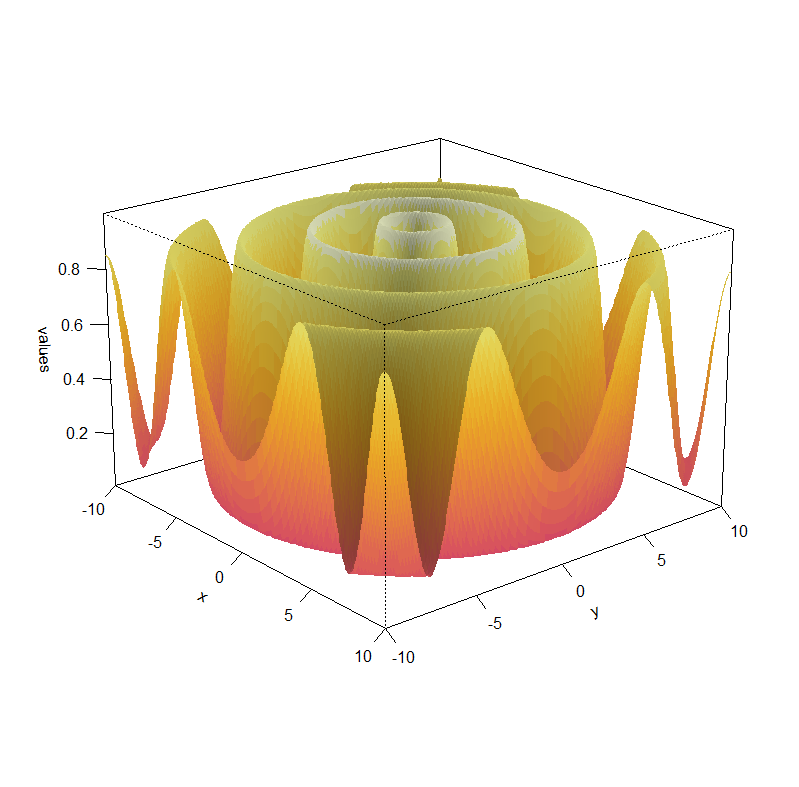
\includegraphics[scale=0.7]{img//roz03//Schaffer1_small_range.png}
%	\caption{Czas wykonania algorytmu HALS w zależności od rzędu faktoryzacji, liczba iteracji wew. 8}
%	\label{fig:HALStime}
%\end{figure}

\begin{equation} \label{eq:Schaffer1}
f(x)=0.5+\frac{\sin^2(x_1^2-x_2^2)-0.5}{[1+0.001(x_1^2+x_2^2)]^2}
\end{equation}


\begin{figure}
\centering
\begin{subfigure}{.5\textwidth}
  \centering
  \includegraphics[width=\linewidth]{{img//roz03//Schaffer1_full_range.png}}
  \caption{ Pełna dziedzina argumentów}
  \label{fig:sub1}
\end{subfigure}%
\begin{subfigure}{.5\textwidth}
  \centering
  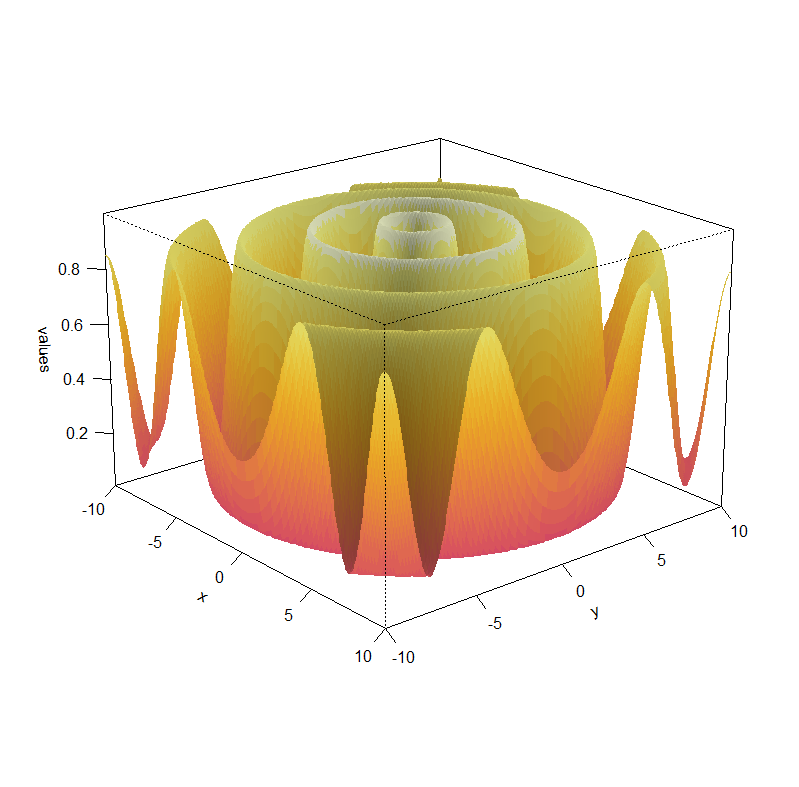
\includegraphics[width=\linewidth]{img//roz03//Schaffer1_small_range.png}
  \caption{Otoczenie ekstremum}
  \label{fig:sub2}
\end{subfigure}
\caption{Przebieg funkcji Schaffer1}
\label{fig:test}
\end{figure}


\subsection{Funkcja Paviani}
\begin{itemize}
\item wzor
\item dziedzina argumentow
\item optimum: jakie i gdzie
\item pewnie cos w necie ciekawego o nim jest
\end{itemize}
\begin{equation}\label{eq:Paviani}
f(x)=\sum_{i=1}^{10} \bigg(\log^2(x_i-2) + \log^2(10-x_i)\bigg) - \left(
\prod_{i=1}^{10} x_i\right)^{0.2}. 
\end{equation}
\section{Opis środowiska testowego}
\begin{itemize}
\item parametry maszyny testowej

\end{itemize}


\section{Przyjęte miary efektywności algorytmów}
\label{sec:przyjete_miary_efektywnosci_algorytmow}
wszstko dla tych samych liczby iteracji
\begin{enumerate}
\item najlepsze znalezione rozwiązanie kolejno w iteracjach
\item średnie rozwiązanie populacji kolejno w iteracjach
\item czas osiągnięcia rozwiązań 90, 95 i 99%

\end{enumerate}
